% Preamble
\documentclass[12pt, a4paper, twoside]{article}
\usepackage[a4paper, left=0.75in, right=0.75in, top=1in, bottom=1in]{geometry}
\usepackage{lipsum, verbatim, fancyhdr, lastpage, graphicx, hyperref, amsmath}
\usepackage[backend=bibtex]{biblatex}
\graphicspath{{./plots/}}
\addbibresource{ref.bib}
% Top Matter
\setlength{\parindent}{0pt}
\hypersetup{
	colorlinks   = true,
	urlcolor     = blue, 
	linkcolor    = blue, 
	citecolor   = red
}
\pagestyle{fancy}
\fancyhead[CO, CE]{GNR 638 (Spring 2024):  Mini Project 2}
\fancyhead[LO, LE, RO, RE]{}
\fancyfoot[CO, CE]{Page \thepage\ of \pageref{LastPage}}
\fancyfoot[LO, LE, RO, RE]{}

\title{\vspace{-0.5in}\textbf{GNR 638 (Spring 2024): Mini Project 2\\{\large Image Deblurring Using Stripformer}}}
\author{Soumen Mondal (23m2157)\\Siddhant Gole (23m2154)\\Akash Pal (23m2158)}
\date{\today}

% Main Matter
\begin{document}
	\maketitle
	\thispagestyle{fancy}
	
	\section{Introduction}
		This project focuses on addressing the challenging task of image deblurring  in computer vision that involves removing the blurring artifacts from images or videos to restore the original, sharp content. The motivation stems from the fact that blurring can be caused by various factors such as camera shake, fast motion, and out-of-focus objects, and can result in a loss of detail and quality in the captured images. The primary objective involves designing a transformer based network architecture, called Stripformer a token-efficient and parameter-efficient transformer model, demanding much less memory usage and computation cost than the vanilla transformer but works better without relying on tremendous training data, with 3.3 million parameters, achieving high accuracy, and ensuring parameter and training time efficiency.
		
	\section{Methodology}
		\subsection{Dataset}
			The dataset utilized for training and evaluation comprises a comprehensive set of sharp images representing 240 distinct object classes, each class encompassing 100 high-resolution images. These images are downscaled to size (H = 256,W = 448). To simulate real-world blurring scenarios, a diverse range of Gaussian kernels is applied to the sharp images, including sizes of $(3 \times 3, 7 \times 7, 11 \times 11)$  with corresponding variance values of (0.3, 1, 1.6), respectively. By convolving these kernels with the sharp images, a corresponding set of blurred images is generated, thus creating a realistic training dataset for image deblurring algorithms. 
		
		\subsection{Model Selection}
		The selection of the Stripformer architecture for image deblurring tasks is driven by its unparalleled balance between performance and resource efficiency. Inspired by the success of transformer-based models, Stripformer is tailored specifically for dynamic scene deblurring challenges. Its innovative design constructs intra- and inter-strip tokens to effectively reweight image features, facilitating the precise identification and correction of region-specific blurred patterns. Among transformer variants, Stripformer stands out for its token and parameter efficiency, ensuring optimal utilization of computational resources while delivering superior deblurring accuracy.
			
	\section{Experimental Setup}
		\subsection{Architecture Details}
			The architecture of Stripformer\cite{paper} for image deblurring tasks encompasses several key components, each playing a vital role in the model's effectiveness and efficiency. The architechture is shown in Figure \ref{F:arc-1} and Figure \ref{F:arc-2}.
			
			\begin{itemize}
				\item \textbf{Feature Embedding Blocks (FEBs):} The Feature Embedding Blocks (FEBs) are meticulously designed to maintain spatial information integrity, ensuring no loss during feature extraction. These blocks are constructed with a combination of convolutional layers and residual blocks, facilitating the generation of feature embeddings essential for subsequent layers' input.
				
				\item \textbf{Intra-SA (Self-Attention) Blocks:} The Intra-SA Blocks in Stripformer are utilized for short-range blur detection, featuring parallel branches dedicated to horizontal and vertical intra-strip attention. These blocks employ a multi-head attention mechanism to reweight features within each strip, enabling them to effectively capture blur patterns with diverse magnitudes and orientations.
				
				\item \textbf{Inter-SA Blocks:} The Inter-SA Blocks in Stripformer are utilized for long-range blur orientation detection, incorporating horizontal and vertical inter-strip attention mechanisms. These blocks employ multi-head attention to capture blur orientations across different scales, enabling adaptive focus on blur patterns with diverse characteristics.

				\item \textbf{Residual Encoder-Decoder Architecture:} The architecture of Stripformer initiates the process by employing Feature Embedding Blocks (FEBs) to generate embedding features. It then integrates convolution layers interleaved with Intra-SA and Inter-SA blocks for effective feature extraction. Upsampling is achieved using transposed convolution, and the model concatenates output features from the encoder with those from the decoder. Finally, residual blocks and a convolution layer are applied to restore sharpness and clarity to the input blurred image.
				
			\end{itemize}
			
			\begin{figure}[hbt!]
				\centering
				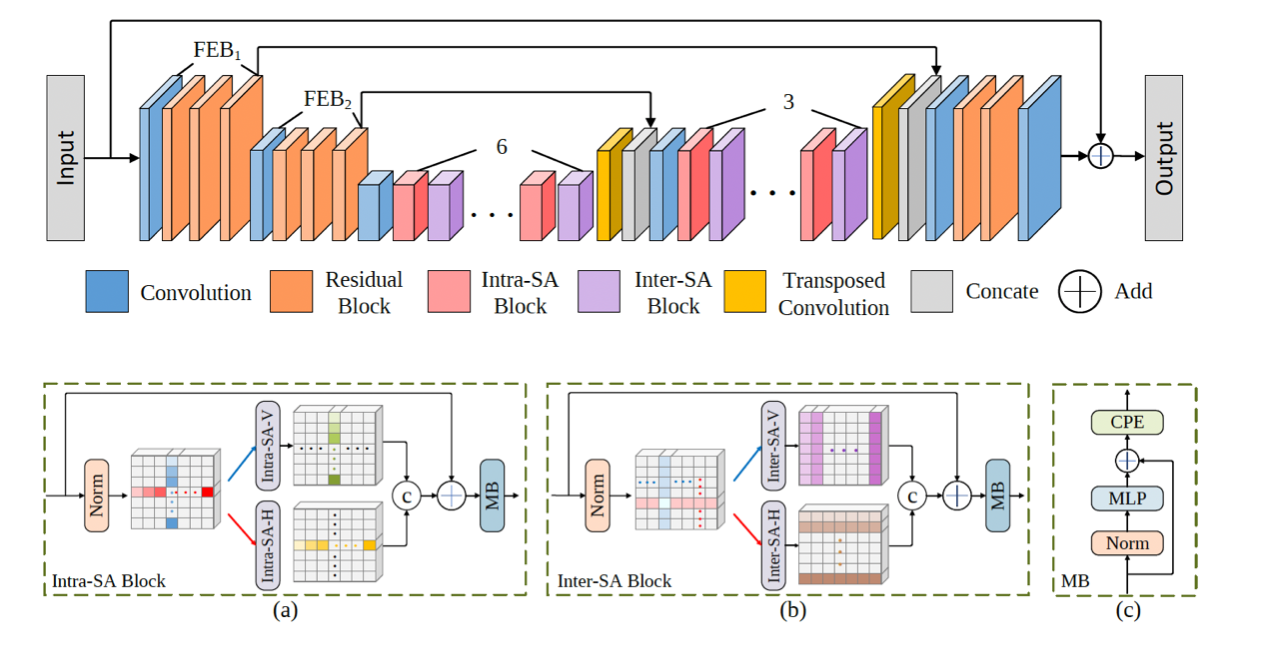
\includegraphics[width=\textwidth]{arc-1}
				\caption{Architecture of Stripformer. (a) Intra-Strip Attention (Intra-SA) Block, (b) Inter-Strip Attention (Inter-SA) Block, where c denotes concatenation, and (c) MLP Block (MB), where CPE denotes the conditional position encoding.}
				\label{F:arc-1}
			\end{figure}
			\begin{figure}[hbt!]
				\centering
				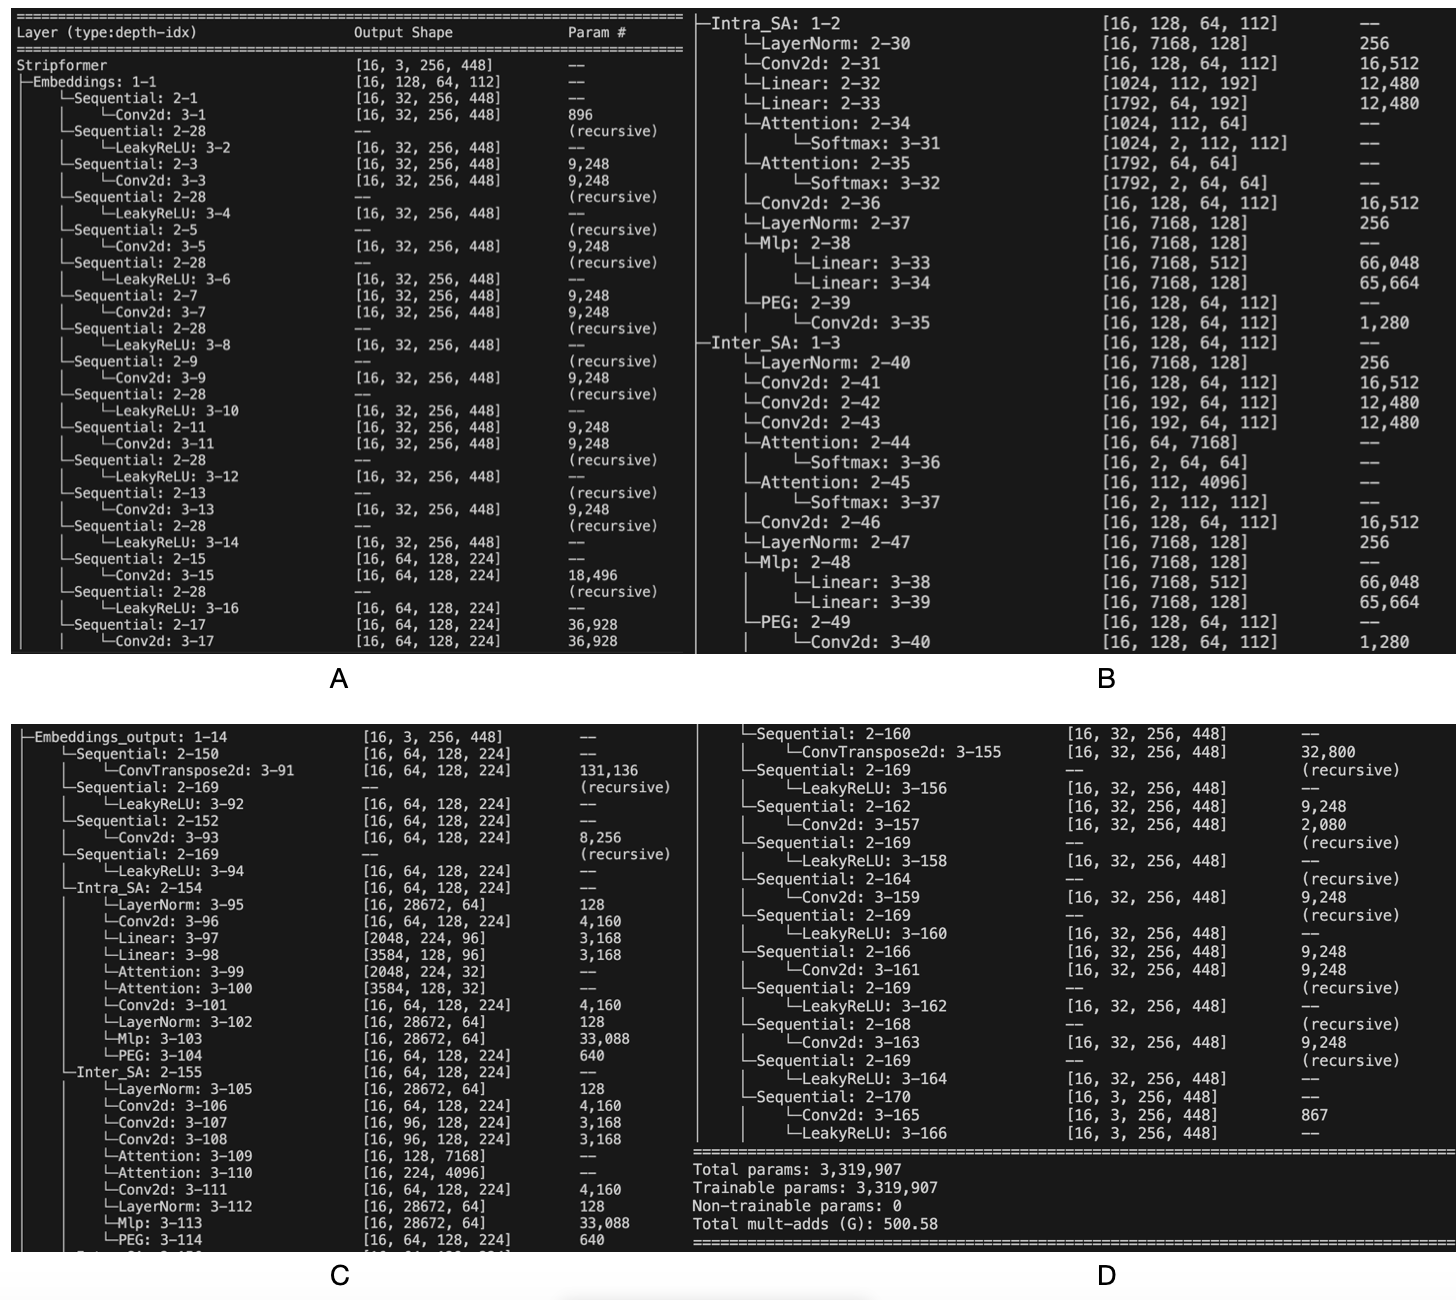
\includegraphics[width=\textwidth]{arc-2}
				\caption{Architecture of Stripformer probed by torchinfo. (A)  A typical embedding block, (B) Interlaced intra SA and inter SA block, (C) Output embedding block where transposed convolution is used, (D) Continuation of output embedding block and total number of parameters of the model.}
				\label{F:arc-2}
			\end{figure}
			
		\subsection{Training Configuration}
			\subsubsection{Batch Size:}
				The batch size refers to the number of samples processed by the model in each training iteration. For Stripformer, we have used a batch size of 16 examples due to the GPU memory constrained of the DGX server as the resource was limited.
				
			\subsubsection{Learning Rate:}
				The learning rate determines the step size at which the model's parameters are updated during training. For Stripformer we have used a fixed learning rate of 0.00001 throughout the training process. No adaptive learning rate schedules were employed for this project.
				
			\subsubsection{Optimizer:}
				The optimizer is responsible for updating the model's parameters based on the computed gradients during backpropagation. For Stripformer, we have utilized the Adam optimizer. Adam optimizer is often favored due to its adaptive learning rate capabilities and effectiveness in training deep neural networks.
				
			\subsubsection{Regularization Techniques:}		
				Regularization techniques are used to prevent overfitting and improve the generalization capability of the model. For Stripformer, we have employed Dropout. Dropout is a technique where randomly selected neurons are ignored during training, reducing the model's reliance on specific features and promoting robustness.  Moreover, early stopping was employed, which involves monitoring the model's performance on a validation set and stopping training when the performance no longer improves, thus preventing overfitting.

		\subsection{Evaluation Metrics}
		Explanation of the evaluation metrics used to assess the model's performance:
		
		\begin{itemize}
			\item \textbf{PSNR (Peak Signal-to-Noise Ratio):} PSNR is a metric commonly used to evaluate the quality of reconstructed images. It measures the ratio between the maximum possible power of a signal and the power of corrupting noise that affects the fidelity of its representation. In the context of image processing, PSNR compares the original image with its reconstruction, providing a quantitative measure of how much the image has been degraded or distorted during the reconstruction process. The higher the PSNR value, the closer the reconstructed image is to the original, indicating better reconstruction quality. PSNR is calculated using the formula:
			
			\begin{equation}
				PSNR = 10 \cdot	\log_{10} \left(\frac{I_{max}^2}{MSE}\right)
			\end{equation}
			
			Where $I_{max}$ is the maximum possible pixel value of the image (e.g., 255 for an 8-bit grayscale image). MSE (Mean Squared Error) is the average squared difference between the pixels of the original and reconstructed images. PSNR is expressed in decibels (dB), and a higher PSNR value indicates a lower level of distortion. It is widely used in image and video processing applications to assess the fidelity of reconstructed images and compare the performance of different reconstruction algorithms.
			
			\item \textbf{Loss:} The loss function described in the context of contrastive learning and deblurring can be broken down into three components:
			
			\begin{enumerate}
				\item Charbonnier Loss (Lchar): The Charbonnier loss is a type of robust loss function commonly used in image processing tasks. It is particularly effective at handling outliers and noise in the data. This loss function measures the difference between the predicted deblurred image and the ground truth sharp image.
				
				\item Edge Loss (Ledge): The edge loss is another component of the loss function used in the deblurring task. It focuses on preserving edge details in the reconstructed image. By penalizing deviations from sharp edges, this loss function helps improve the perceptual quality of the deblurred output.
				
				\item Contrastive Loss (Lcon): The contrastive loss is a key component inspired by contrastive learning techniques. It encourages the deblurred output to be similar to the ground truth sharp image while being dissimilar to the blurred input image. This is achieved by pulling the features of the deblurred image close to the features of the sharp image (positive samples) while pushing them away from the features of the blurred input image (negative samples) in a latent feature space.
			\end{enumerate}
			
			The overall loss function for the deblurring task combines these three components with respective weighting factors $\lambda_1$ and $\lambda_2$. By optimizing this loss function during training, the model learns to produce deblurred images that are visually similar to the ground truth while also being distinct from the blurred input, thus improving the quality of the deblurring process. Adjusting the weighting factors allows for fine-tuning the balance between the different loss components based on their relative importance in the task.
		\end{itemize}
		
	\section{Results}
		\subsection{Training Process}
			The training process of Stripformer involved monitoring both the training loss and PSNR over epochs to assess the model's convergence and performance. Figure \ref{F:train} and \ref{F:val} illustrates the training and validation curves plotted against the number of optimizer steps. As shown in the figure, both the training loss and PSNR demonstrate a decreasing trend over epochs, indicating that the model is learning from the training data and improving its performance.
			\\
			\\
			The training loss steadily decreases, while the training PSNR gradually increases, suggesting that the model is effectively minimizing its prediction errors and learning to reconstruct or deblur the blurred images more accurately. Additionally, the convergence of both loss and PSNR curves indicates that the model is stable and not overfitting to the training data. See Table \ref{T:train} for training details.
			
			\begin{figure}[hbt!]
				\centering
				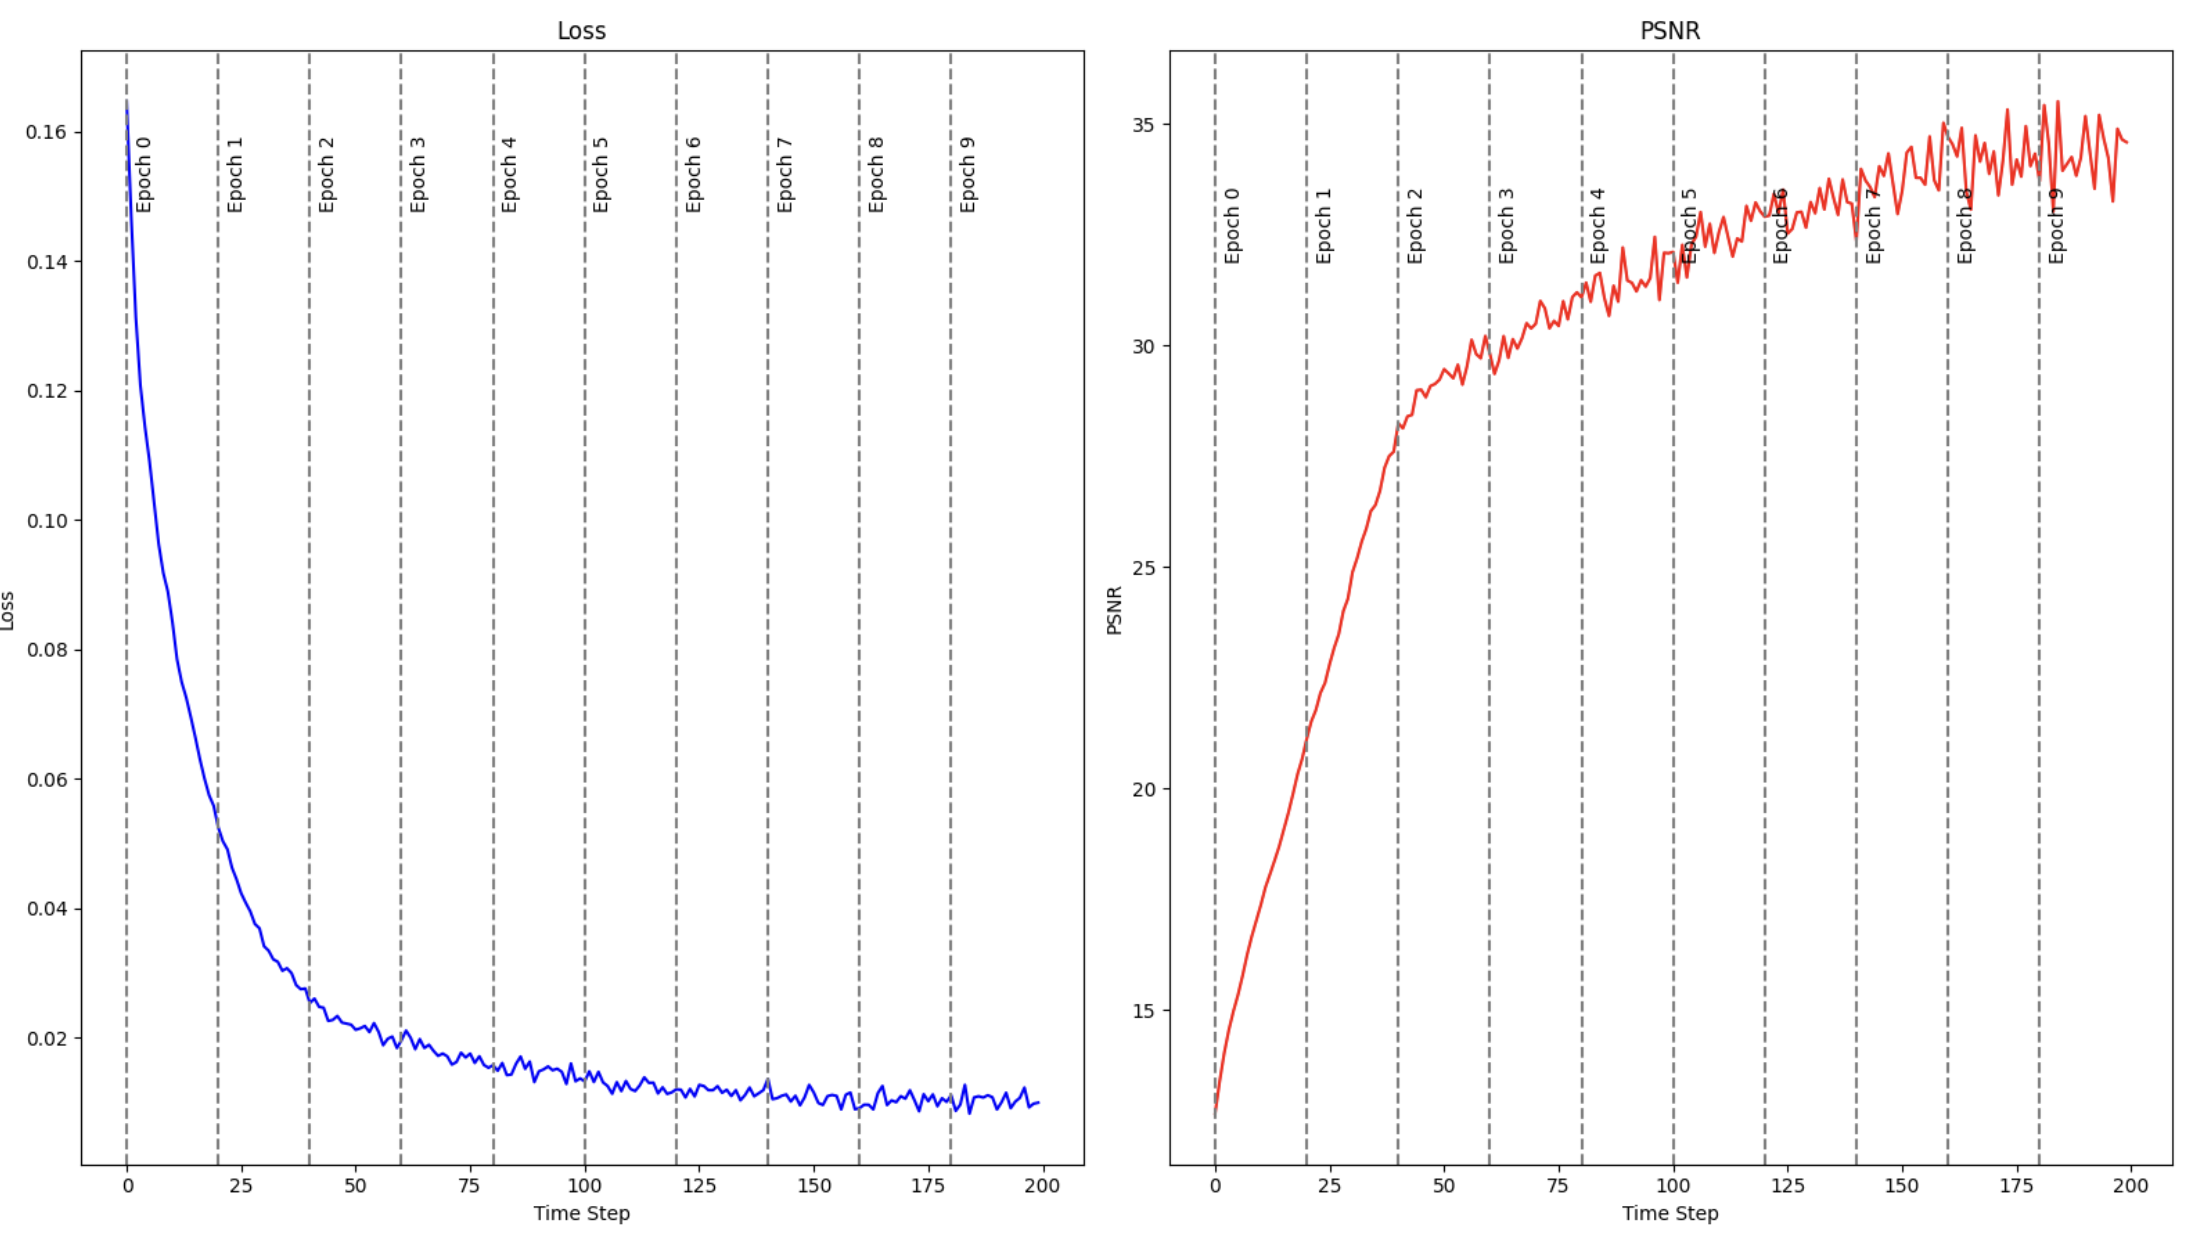
\includegraphics[width=0.8\textwidth]{train.png}
				\caption{Training Loss and PSNR Curves of Stripformer for 10 epochs.}
				\label{F:train}
			\end{figure}
			
			\begin{figure}[hbt!]
				\centering
				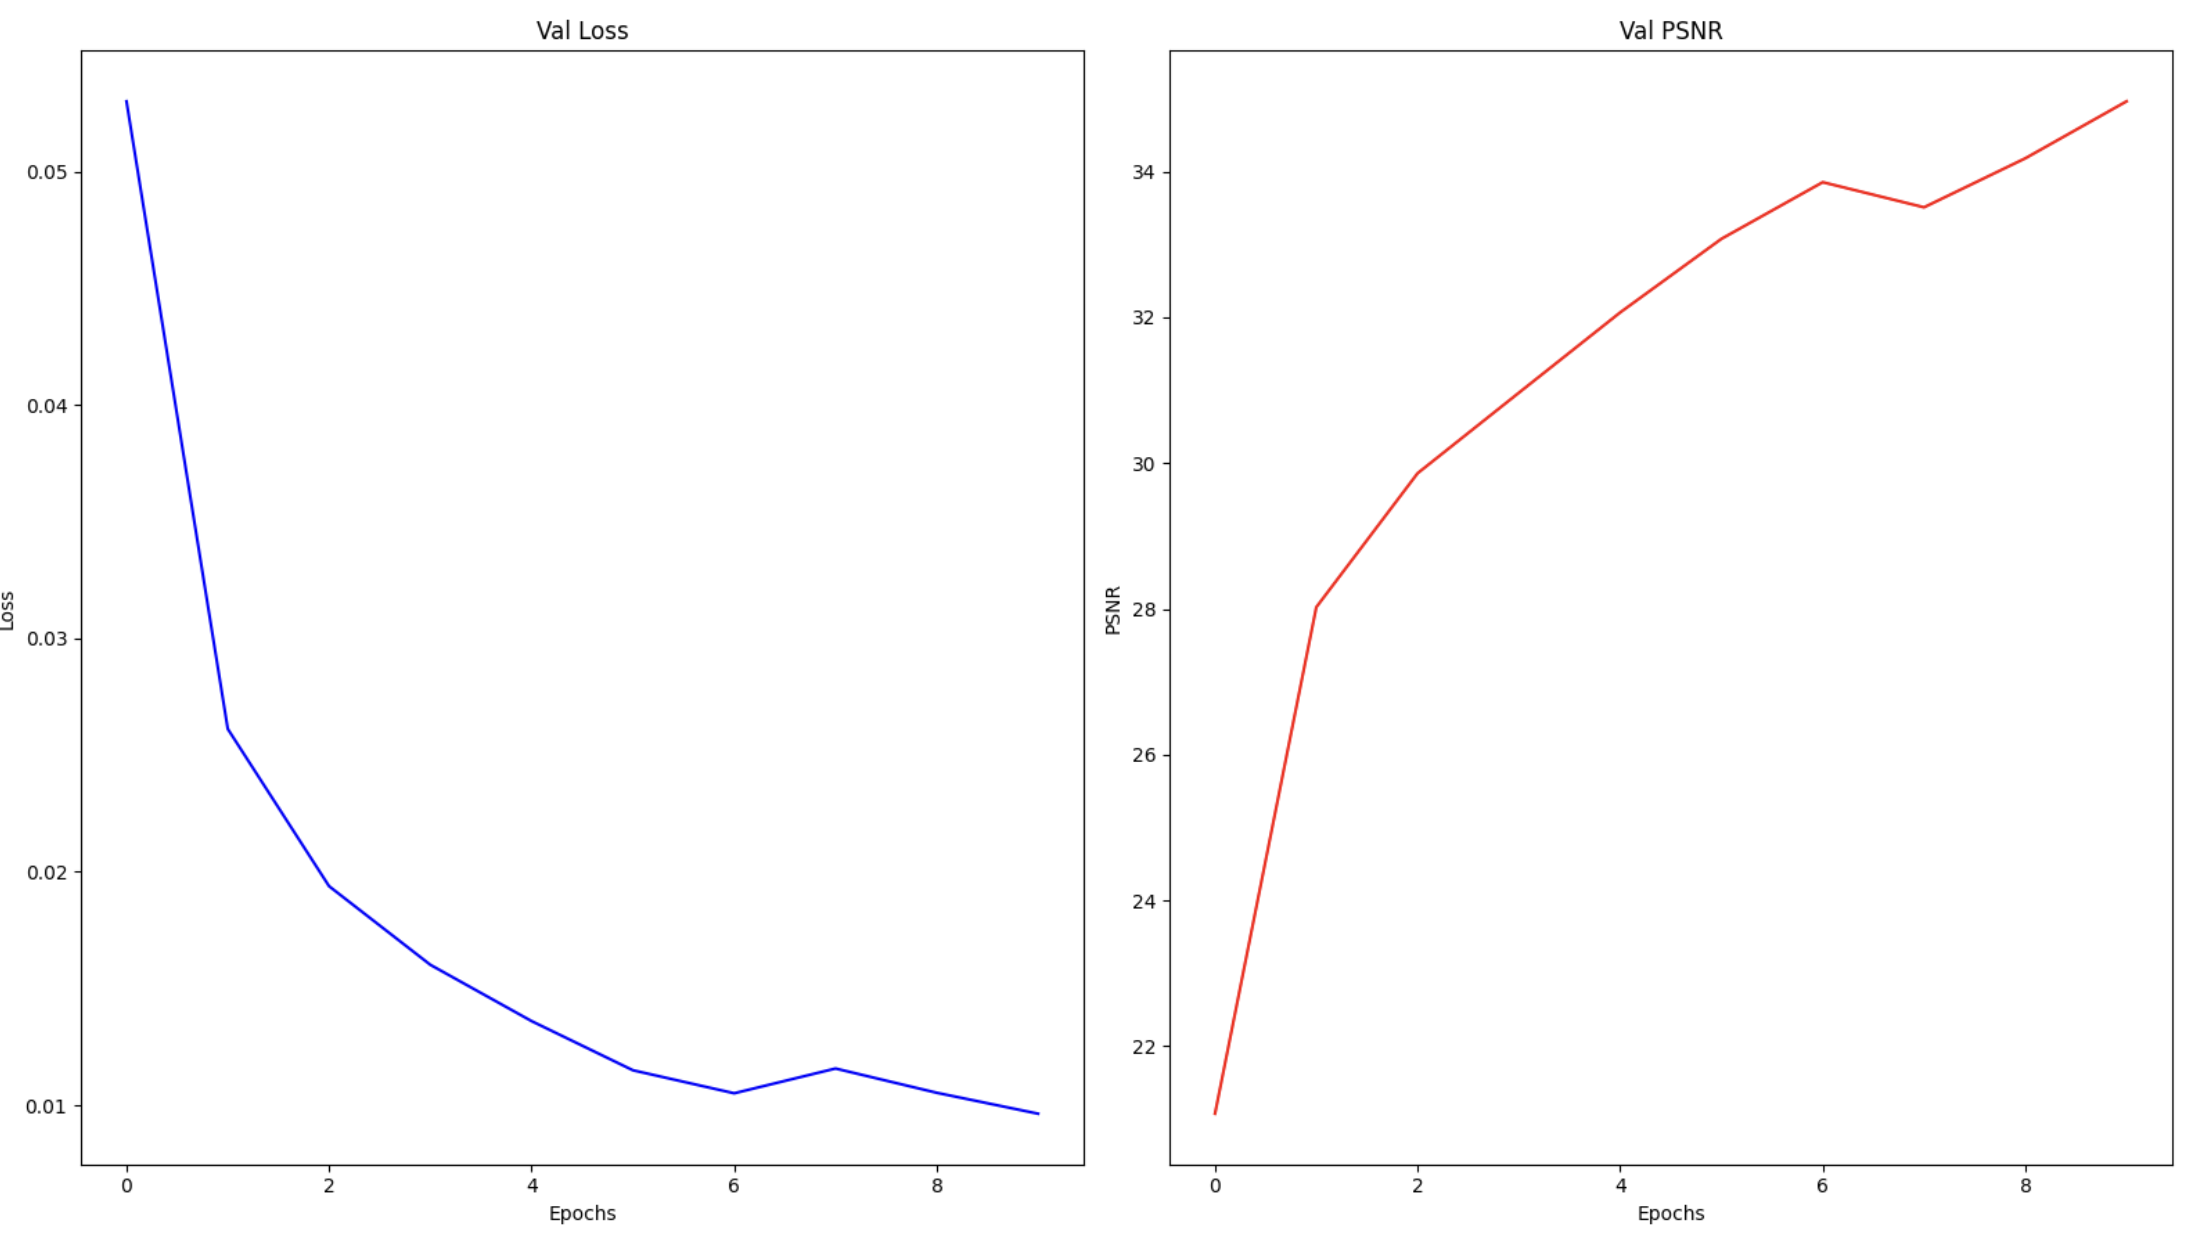
\includegraphics[width=0.8\textwidth]{val.png}
				\caption{Validation Loss and PSNR Curves of Stripformer for 10 epochs.}
				\label{F:val}
			\end{figure}
		
		\subsection{Performance Evaluation}
			After training, the performance of Stripformer was evaluated on the test set to assess its PSNR in reconstructing unseen blurred data. The final test PSNR achieved on the test set was \textbf{24.02 dB}, indicating that the model generalizes decently to new examples. The value of test PSNR could be attributed due to that fact that the test set could have been taken from a different blurring distribution.
			\\
			\\	
			Overall, the results of the training process and performance evaluation highlight the success of Stripformer in achieving high PSNR while maintaining parameter efficiency, making it a suitable choice for various computer vision tasks. See Table \ref{T:test} for testing details.
			
			\begin{table}
				\begin{center}
					\begin{tabular}{c c c c c c}
						\hline
						\textbf{Model Name}& \textbf{\# of Parameters} & \textbf{Train Loss} & \textbf{Train PSNR} & \textbf{Val Loss} & \textbf{Val PSNR} \\ \hline
						Stripformer & $3.32$ Million & $0.012$ & $35.43$ dB & $0.017$ & $36.41$ dB \\ \hline
					\end{tabular}
					\caption{Deblurring Results on Train and Validation Set for Best Epoch \#9}\label{T:train}
				\end{center}
			\end{table}
			
			\begin{table}
				\begin{center}
						\begin{tabular}{c c c c}
								\hline
								\textbf{Model Name} & \textbf{\# of Parameters} & \textbf{Test Loss} & \textbf{Test PSNR} \\ \hline
								Stripformer & $3.32$ Million & $0.021$ & $24.02$ dB \\ \hline
							\end{tabular}
						\caption{Deblurring Results on Test Set}\label{T:test}
					\end{center}
			\end{table}
			
		\subsection{Relevant Links of Results}
			The following links provide access to various resources related to the results of our experiments:
			
			\begin{itemize}
				\item \textbf{Best Model Checkpoint:} The checkpoint file for best performing model can be accessed on \url{https://github.com/soumenkm/GNR-638-miniproject2/blob/main/outputs/model_best_epoch.pth}
				
				\item \textbf{Code:} The Python files for training, validation, testing and plotting can be found on \url{https://github.com/soumenkm/GNR-638-miniproject2/tree/main}
				
				\begin{itemize}
					\item data\_preprocess.py: Contains functions for preprocessing data, such as resizing images or performing data augmentation, before training the model.
					
					\item blur\_dataset.py:
					Defines the BlurDataset class used for loading and preprocessing blur images and their corresponding sharp images for training or evaluation.
					
					\item Stripformer\_arch.py:
					Contains the architecture of the Stripformer model, including the definition of transformer blocks.
					
					\item loss\_function.py: Defines custom loss functions used during the training of the Stripformer model, such as Charbonnier loss, edge loss, and contrastive loss.
					
					\item train\_subset.py: Contains functions or scripts for training the Stripformer model on a subset of the training data, useful for debugging or experimentation purposes.
					
					\item plot\_train\_details.py: Contains functions or scripts for plotting and visualizing the training details, such as loss curves, PSNR values, etc., during or after training.			
					
					\item test.py: Includes functions or scripts for testing the functionality of the model for test set.
					
					\item eval.py: Includes functions or scripts for evaluating the performance of the trained model on a separate test dataset, calculating metrics like PSNR.
					
				\end{itemize}

			\end{itemize}

	\section{Conclusion}
		In conclusion, the experimentation with Stripformer for the deblurring task yielded promising results. Through rigorous training and evaluation, the model showcased commendable performance in both convergence during training and PSNR on the train set. The decreasing trend observed in both training loss and increasing trend in PSNR over epochs indicate effective learning without overfitting, corroborated by the stable convergence of loss and PSNR curves.
		\\
		\\
		Upon evaluation on the test set, Stripformer demonstrated its capability by achieving a final PSNR of 24.02 dB. These findings underscore the significance of informed model selection and highlight the effectiveness of Stripformer in addressing deblurring challenges. Moving forward, the insights gained from this study can inform future research and application of Stripformer models in various computer vision domains.
	
	\printbibliography
\end{document}